\documentclass[journal,12pt,twocolumn]{IEEEtran}

\usepackage{setspace}
\usepackage{gensymb}
\singlespacing
\usepackage[cmex10]{amsmath}
\usepackage{cancel}
\usepackage{amsthm}
\usepackage{amsmath}
\usepackage{paralist}
\usepackage{upgreek}
\usepackage{mathrsfs}
\usepackage{txfonts}
\usepackage{stfloats}
\usepackage{bm}
\usepackage{cite}
\usepackage{cases}
\usepackage{subfig}

\usepackage{longtable}
\usepackage{multirow}
\usepackage{enumitem}
\usepackage{mathtools}
\usepackage{steinmetz}
\usepackage{tikz}
\usepackage{circuitikz}
\usepackage{verbatim}
\usepackage{tfrupee}
\usepackage[breaklinks=true]{hyperref}
\usepackage{graphicx}
\usepackage{tkz-euclide}

\usetikzlibrary{calc,math}
\usepackage{listings}
    \usepackage{color}                                            %%
    \usepackage{array}                                            %%
    \usepackage{longtable}                                        %%
    \usepackage{calc}                                             %%
    \usepackage{multirow}                                         %%
    \usepackage{hhline}                                           %%
    \usepackage{ifthen}                                           %%
    \usepackage{lscape}     
\usepackage{multicol}
\usepackage{chngcntr}

\DeclareMathOperator*{\Res}{Res}
\usepackage{romannum}
\renewcommand\thesection{\arabic{section}}
\renewcommand\thesubsection{\thesection.\arabic{subsection}}
\renewcommand\thesubsubsection{\thesubsection.\arabic{subsubsection}}

\renewcommand\thesectiondis{\arabic{section}}
\renewcommand\thesubsectiondis{\thesectiondis.\arabic{subsection}}
\renewcommand\thesubsubsectiondis{\thesubsectiondis.\arabic{sub subsection}}


\hyphenation{optical networks semiconduc-tor}
\def\inputGnumericTable{}                                 %%

\lstset{
%language=C,
frame=single, 
breaklines=true,
columns=fullflexible
}
\date{March 2021}

\begin{document}
\newcommand{\multlinecomment}[1]{\directlua{-- #1}}
\newcommand{\BEQA}{\begin{eqnarray}}
\newcommand{\EEQA}{\end{eqnarray}}
\newcommand{\define}{\stackrel{\triangle}{=}}
\bibliographystyle{IEEEtran}
\raggedbottom
\setlength{\parindent}{0pt}
\providecommand{\mbf}{\mathbf}
\providecommand{\pr}[1]{\ensuremath{\Pr\left(#1\right)}}
\providecommand{\qfunc}[1]{\ensuremath{Q\left(#1\right)}}
\providecommand{\fn}[1]{\ensuremath{f\left(#1\right)}}
\providecommand{\e}[1]{\ensuremath{E\left(#1\right)}}
\providecommand{\sbrak}[1]{\ensuremath{{}\left[#1\right]}}
\providecommand{\lsbrak}[1]{\ensuremath{{}\left[#1\right.}}
\providecommand{\rsbrak}[1]{\ensuremath{{}\left.#1\right]}}
\providecommand{\brak}[1]{\ensuremath{\left(#1\right)}}
\providecommand{\lbrak}[1]{\ensuremath{\left(#1\right.}}
\providecommand{\rbrak}[1]{\ensuremath{\left.#1\right)}}
\providecommand{\cbrak}[1]{\ensuremath{\left\{#1\right\}}}
\providecommand{\lcbrak}[1]{\ensuremath{\left\{#1\right.}}
\providecommand{\rcbrak}[1]{\ensuremath{\left.#1\right\}}}
\theoremstyle{remark}
\newtheorem{rem}{Remark}
\newcommand{\sgn}{\mathop{\mathrm{sgn}}}
\providecommand{\abs}[1]{\vert#1\vert}
\providecommand{\res}[1]{\Res\displaylimits_{#1}} 
\providecommand{\norm}[1]{\lVert#1\rVert}
%\providecommand{\norm}[1]{\lVert#1\rVert}
\providecommand{\mtx}[1]{\mathbf{#1}}
\providecommand{\mean}[1]{E[ #1 ]}
\providecommand{\fourier}{\overset{\mathcal{F}}{ \rightleftharpoons}}
%\providecommand{\hilbert}{\overset{\mathcal{H}}{ \rightleftharpoons}}
\providecommand{\system}{\overset{\mathcal{H}}{ \longleftrightarrow}}
	%\newcommand{\solution}[2]{\textbf{Solution:}{#1}}
\newcommand{\solution}{\noindent \textbf{Solution: }}
\newcommand{\cosec}{\,\text{cosec}\,}
\providecommand{\dec}[2]{\ensuremath{\overset{#1}{\underset{#2}{\gtrless}}}}
\newcommand{\myvec}[1]{\ensuremath{\begin{pmatrix}#1\end{pmatrix}}}
\newcommand{\mydet}[1]{\ensuremath{\begin{vmatrix}#1\end{vmatrix}}}
\numberwithin{equation}{subsection}
\makeatletter
\vspace{3cm}
\title{Gate Assignment}
\author{RONGALA ARUN SIDDARDHA - AI20BTECH11019}
\maketitle
\newpage
\bigskip
\renewcommand{\thetable}{\theenumi}

%
Download latex code from 
%
\begin{lstlisting}
https://github.com/ArunSiddardha/EE900/tree/main/Gate_assignment/Gate_Assignment.tex
\end{lstlisting}

\section*{GATE-EC 2009 Q.41}
Consider a system whose input x and input y are related by the equation,
$$y\brak{t}=\int_{-\infty}^{\infty}x\brak{t-\uptau}h\brak{2\uptau}d\uptau$$
where h\brak{t} is shown in the graph.
Which of the following properties are possesed by the system?\\
BIBO : Bounded input gives a bounded output\\
casual: the system is casual\\
LP: The system is low pass\\
LTI : The system is linear and time-variant\\
\begin{figure}[htp]
    \centering
    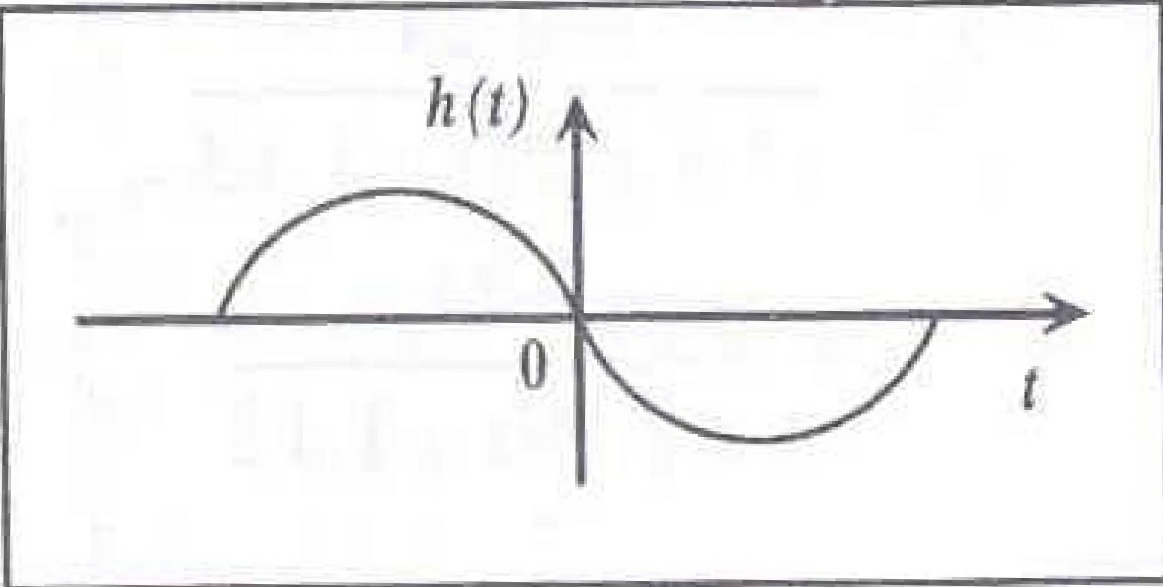
\includegraphics[width =0.8\columnwidth]{Graph.jpg}
    \caption{$h\brak{t}$}
    \label{fig:my_label}
\end{figure}
\begin{enumerate}
    \item Casual,LP 
    \item BBIO, LTI
    \item BIBO,casual,LTI
    \item LP,LTI
\end{enumerate}
\section*{SOLUTION}
\textbf{Answer: 2}\\
Lets take \textbf{h(t)} as sin(t) in the interval of - $\pi$ to $\pi$.

\textbf{LTI:}\\
We say that a system is\textbf{ linear} if and only if it follows the Principle of Superposition, i.e Law of Additivity and Law of Homogeneity.\\
A system is said to be \textbf{time invariant} if the output signal does not depend on the absolute time, i.e a time delay on the input signal directly equates to the delay in the output signal.
\label{T}

The system relating the input signal $x(t$) and output signal $y(t)$, given by 
\begin{align}
     y\brak{t}=\int_{-\infty}^{\infty}x\brak{t-\uptau}h\brak{2\uptau}d\uptau \label{L}
\end{align}
is linear and time invariant in nature.


From \eqref{L}, we can say the system is linear if it follows both the laws of Additivity and Homogeneity.\\
\textbf{Law of Additivity:}\\
Let the two input signals be $x_1(t)$ and $x_2(t)$, and their corresponding output signals be $y_1(t)$ and $y_2(t)$, then:
\begin{align}
    y_{1}\brak{t}&=\int_{-\infty}^{\infty}x_{1}\brak{t-\uptau}h\brak{2\uptau}d\uptau\\
    y_{2}\brak{t}&=\int_{-\infty}^{\infty}x_{2}\brak{t-\uptau}h\brak{2\uptau}d\uptau \\
    y_1(t) + y_2(t) &= \int_{t-T}^t[x_{1}\brak{t-\uptau}h\brak{2\uptau} + x_{2}\brak{t-\uptau}h\brak{2\uptau}]\,d\uptau
    \label{1}
\end{align}
Now, consider the input signal of $x_1(t) + x_2(t)$, then the corresponding output signal is given by $y'(t)$:
\begin{align}
    y'(t) = \int_{t-T}^t[x_{1}\brak{t-\uptau}h\brak{2\uptau} + x_{2}\brak{t-\uptau}h\brak{2\uptau}]\,d\uptau
    \label{2}
\end{align}
Clearly, from \eqref{1} and \eqref{2}:
\begin{align}
    y'(t) = y_1(t) + y_2(t)
\end{align}
Thus, the Law of Additivity holds.\\
\textbf{Law of Homogeneity: }\\
Consider an input signal $kx(t)$, where $k$ is any constant. Let the corresponding output be given by $y'(t)$, then:
\begin{align}
    y'(t) = \int_{-\infty}^{\infty}kx\brak{t-\uptau}h\brak{2\uptau}d\uptau\\
    = k\int_{-\infty}^{\infty}x\brak{t-\uptau}h\brak{2\uptau}d\uptau\\
     = ky(t)
     \label{3}
\end{align}
Clearly, from \eqref{3},
\begin{align}
    y'(t) = ky(t)
\end{align}
Thus, the Law of Homogeneity holds.\\
Since both the Laws hold, the system satisfies the Principle of Superposition, and is thus, a \textbf{linear system}.\\



\textbf{BIBO:}\\
We say that a system is BIBO stable if bounded input $x \brak{t}$ gives bounded input $y\brak{t}$.
Here since $h\brak{t}$ is bounded if we give a bounded input $x\brak{t}$ and the integral is also is in betweeen two bounded inputs so we get a bounded value of $y\brak{t}$.
So the system is \textbf{BIBO stable}.\\

 Therefore, The answer is \textbf{option 2}
 \section*{LAPLACE}
Taking the laplace transform form for the h(t)
\begin{align}
    H(s)= \int_{0}^{\infty} h(t) e^{-st} dt\\
    H(s)= \int_{0}^{\infty} -sin(t) e^{-st} dt \\
    H(s)= -\frac{-cos(t)+ssin(t)}{1+s^2} e^{-st} \bigg\rvert^{\infty}_{0}\\
    H(s) = -\brak{0 - \frac{1-0}{1+s^2}}\\
    H(s) = \frac{1}{1+s^2}
\end{align}
\begin{figure}
    \centering
    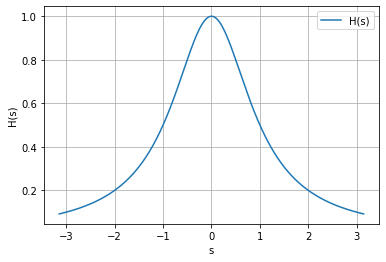
\includegraphics[width = \columnwidth]{Figure.png}
    \caption{Laplace transform}
    \label{fig:my_label}
\end{figure}
The laplace transform of the above function also posses BBIO(because bounded input produces bounded output),LTI(trivial) properties.\\
So for the laplace transform also \textbf{option 2 is correct}

\section*{CONVOLUTION}
 $y(t)$ is defined as convolution of g(t) and x(t) $ (taking \; h(2\uptau)\; as\; g(\uptau)$ $\because h(t) \;is \; -\sin(t) \implies g(t) \;is\; -sin(2t)$)
\begin{align}
    y(t) = g(t) * x(t) 
\end{align}
The convolution of the y(t) holds the following properties 
\begin{enumerate}
    \item  \textbf{Commutative property :}  For the input function $x(t)$ , and LTI system responses $g(t)$  the following expression is valid:\\
    $x(t)*g(t)=g(t)*x(t)=\int_{-\infty}^{\infty}f(t–\uptau)g(\uptau)d\uptau$
    \item  \textbf{Distributive property :}
    For the input function $x(t)$ , and LTI system response $g_1(t), g_2(t)$  the following expression is valid:\\ $x(t)*(g_1(t)+g_2(t))=x(t)*g_1(t)+x(t)*g_2(t)$
    \item  \textbf{Associative property:}
    For the input functions $x(t)$ , and LTI system responses $g_1(t), g_2(t)$  the following expressions are valid:\\ $x(t)*(g_1(t)*g_2(t))=(x(t)*g_1(t))*g_2(t)$
    \item \textbf{Inversion property:}
    If the LTI system is an inverting function, then $g_1(t)*g_2(t)=\delta(t) $, here $g_1(t), g_2(t)$ are responses of the input and output functions in the case of continuous-time functions.
    \item \textbf{Stability property:}
    Let’s assume that the input function is limited, so $x(t)<A$, then considering the convolution integral we can understand if the output function is stable. $y(t)<\int_{-\infty}^{\infty} Ag(\uptau)d\uptau$, so the output function $y(t)$ will be stable if the integral $\int_{-\infty}^{\infty} g(\uptau)d\uptau < \infty$. $\because \text{Here} \; g(t) \; \text{is an odd function the integral}$ becomes 0.So the system is stable here.
\end{enumerate}
\end{document}
